% Propósito: evitar la representación de la conducción ósea como una única
% ruta que omite por completo el oído externo y el medio.
% Origen: cinco contribuciones funcionales enumeradas en la sección
% \ref{sec:u6-conduccion-osea}. Esquema conceptual; no expresa magnitudes ni
% importancia relativa.
% Descripción accesible: una vibración aplicada al cráneo o a los tejidos se
% divide en cinco rutas paralelas: radiación hacia el canal, inercia osicular,
% inercia de fluidos, deformación de la cápsula y transmisión por tejidos y
% cavidades. Todas convergen en diferencias de presión y movimiento de la
% partición coclear. Una nota aclara que actúan simultáneamente y con peso
% dependiente de frecuencia, punto de estimulación y acoplamiento.
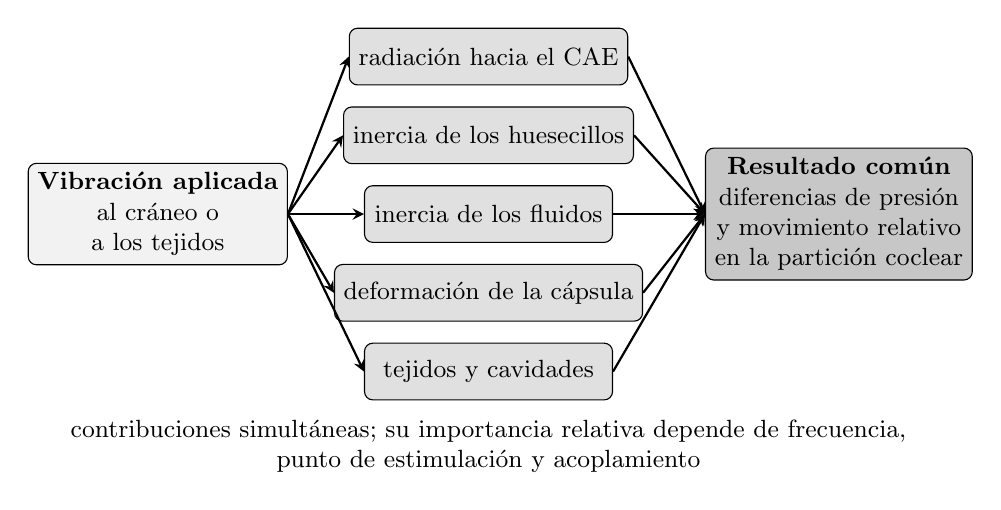
\begin{tikzpicture}[font=\small,>=stealth,x=1cm,y=1cm]
    \tikzset{
        source/.style={
            draw,rounded corners=3pt,fill=black!5,
            minimum width=2.45cm,minimum height=1.25cm,align=center
        },
        route/.style={
            draw,rounded corners=3pt,fill=black!12,
            minimum width=3.15cm,minimum height=0.72cm,align=center
        },
        result/.style={
            draw,rounded corners=3pt,fill=black!22,
            minimum width=2.65cm,minimum height=1.45cm,align=center
        },
        flow/.style={->,thick}
    }

    \node[source] (input) at (1.35,2.75)
        {\textbf{Vibración aplicada}\\al cráneo o\\a los tejidos};

    \node[route] (cae) at (5.55,4.75) {radiación hacia el CAE};
    \node[route] (oss) at (5.55,3.75) {inercia de los huesecillos};
    \node[route] (fluid) at (5.55,2.75) {inercia de los fluidos};
    \node[route] (capsule) at (5.55,1.75) {deformación de la cápsula};
    \node[route] (tissue) at (5.55,0.75) {tejidos y cavidades};

    \node[result] (output) at (10.00,2.75)
        {\textbf{Resultado común}\\diferencias de presión\\y movimiento relativo\\
         en la partición coclear};

    \foreach \n in {cae,oss,fluid,capsule,tissue}{
        \draw[flow] (input.east) -- (\n.west);
        \draw[flow] (\n.east) -- (output.west);
    }

    \node[align=center] at (5.55,-0.20)
        {contribuciones simultáneas; su importancia relativa depende de
         frecuencia,\\punto de estimulación y acoplamiento};
\end{tikzpicture}
